\documentclass[12pt]{article}
\usepackage[utf8]{inputenc}
\usepackage{float}
\usepackage{amsmath}


\usepackage[hmargin=3cm,vmargin=6.0cm]{geometry}
%\topmargin=0cm
\topmargin=-2cm
\addtolength{\textheight}{6.5cm}
\addtolength{\textwidth}{2.0cm}
%\setlength{\leftmargin}{-5cm}
\setlength{\oddsidemargin}{0.0cm}
\setlength{\evensidemargin}{0.0cm}

%misc libraries goes here
\usepackage{tikz}
\usetikzlibrary{automata,positioning}

\begin{document}

\section*{Student Information } 
%Write your full name and id number between the colon and newline
%Put one empty space character after colon and before newline
Full Name : Alper KOCAMAN\\
Id Number : 2169589 \\

% Write your answers below the section tags
\section*{Answer 1}

\subsection*{a.}

The set of rational numbers inside the open interval (-1,0) can be groupped by looking the sum of absolute values of both dividend and denominator.\\
$\frac{-1}{2} $(index 1) $\rightarrow sum=3$; \\
$\frac{-1}{3} $(index 2) $\rightarrow sum=4$; \\ 
$\frac{-1}{4} $(index 3)$ ,\frac{-2}{3} $(index 4)  $\rightarrow sum=5$; \\
$\frac{-1}{5} $(index 5)$ ,\frac{-2}{4} $(index 6)  $\rightarrow sum=6$; \\ 
$\frac{-1}{6} $(index7)  $,\frac{-2}{5} $(index 8)  ,$\frac{-3}{4}$ (index 9)  $\rightarrow sum=7$ ...\\

As done in positive rational numbers,we can map natural numbers to rational numbers in the open interval (-1,0).By ordering them in the ascending order of sum of both values, numbers can be indexed.Indexing of first nine is above.\\

Thus, every rational number inside $(-1,0)$ can appear somewhere in the list and it is possible to create a bijection relation between these group and natural numbers.So, these group is countable.\\

However,there is infinitely many rational numbers betwwen this interval.\\

Thus,the set of rational numbers inside the open interval (-1,0) is countably infinite.\\

\subsection*{b.}

Let $L_1$ and $L_2$ are regular languages.\\
Then $L_1 \cup L_2$, $L_1 o L_2$ and ${L_1}^*$ are also regular languages.\\ 
A language is regular if it is finite language.So,in this question,L is finite language and it is regular.\\
Thus,$L^+ = L o L^*$ is regular.\\
So,the set D is empty and $|D|= 0$.


\subsection*{c.}

A language is regular iff it is accepted by a finite automaton.So,if a language cannot be recognized by any Finite Automaton, this language is not a regular language.\\

So,the set of all languages on the binary alphabet $\Sigma = \{a,b\} $ which cannot be recognized by any finite automaton is set of not regular languages.\\ 
 
The set of all languages on the binary alphabet $\Sigma = \{a,b\} $ is $2^{\Sigma^*} $ which is the all possible subsets of $\Sigma^*$.Since the all possible subsets of a countably infinite set is uncountably infinite,$2^{\Sigma^*} $ is uncountably infinite.Only $\Sigma^*$ of them are regular languages and this set is countably infinite.The rest are nonregular languages and the set of all nonregular languages on the binary alphabet $\Sigma = \{a,b\} $ is uncountably infinite.

\section*{Answer 2}

\subsection*{a.}

\begin{center}
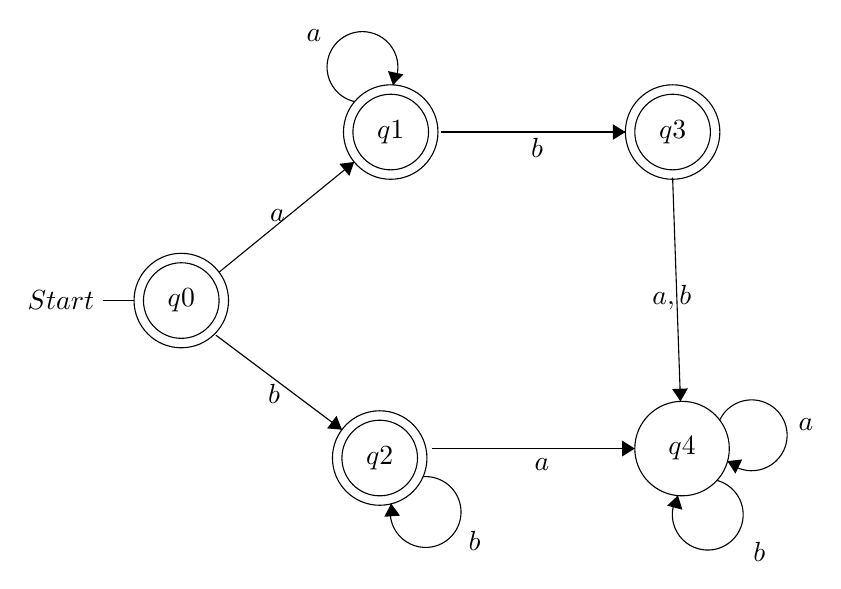
\begin{tikzpicture}[scale=0.2]
\tikzstyle{every node}+=[inner sep=0pt]
\draw [black] (15.1,-26.6) circle (3);
\draw (15.1,-26.6) node {$q0$};
\draw [black] (15.1,-26.6) circle (2.4);
\draw [black] (28.4,-15.9) circle (3);
\draw (28.4,-15.9) node {$q1$};
\draw [black] (28.4,-15.9) circle (2.4);
\draw [black] (27.7,-36.6) circle (3);
\draw (27.7,-36.6) node {$q2$};
\draw [black] (27.7,-36.6) circle (2.4);
\draw [black] (46.3,-15.9) circle (3);
\draw (46.3,-15.9) node {$q3$};
\draw [black] (46.3,-15.9) circle (2.4);
\draw [black] (46.9,-36) circle (3);
\draw (46.9,-36) node {$q4$};
\draw [black] (17.5,-24.8) -- (26.08,-17.8);
\draw (21.7,-21.23) node [left] {$a$};
\fill [black] (26.08,-17.8) -- (25.14,-17.92) -- (25.77,-18.69);
\draw [black] (17.3,-28.8) -- (25.3,-34.8);
\draw (21.4,-32.5) node [left] {$b$};
\fill [black] (25.3,-34.8) -- (24.96,-33.92) -- (24.36,-34.72);
\draw [black] (31.6,-15.9) -- (43.3,-15.9);
\draw (38.1,-16.9) node [left] {$b$};
\fill [black] (43.3,-15.9) -- (42.5,-15.4) -- (42.5,-16.4);
\draw [black] (46.3,-18.8) -- (46.8,-33);
\draw (46.25,-27.23) node [above] {$a,b$};
\fill [black] (46.8,-33) -- (47.27,-32.18) -- (46.27,-32.22);
\draw [black] (31,-36) -- (43.9,-36);
\draw (38.5,-37) node [left] {$a$};
\fill [black] (43.9,-36) -- (43.1,-35.5) -- (43.1,-36.5);
\draw [black] (26.119,-13.97) arc (257.49857:-30.50143:2.25);
\draw (23.52,-10.18) node [above] {$a$};
\fill [black] (28.54,-12.92) -- (29.21,-12.24) -- (28.23,-12.03);
\draw [black] (30.443,-37.785) arc (94.36454:-193.63546:2.25);
\draw (33.73,-41.23) node [below] {$b$};
\fill [black] (28.43,-39.5) -- (27.99,-40.33) -- (28.99,-40.26);
\draw [black] (49.285,-34.199) arc (154.7843:-133.2157:2.25);
\draw (54.26,-34.45) node [right] {$a$};
\fill [black] (49.78,-36.8) -- (50.29,-37.59) -- (50.72,-36.69);
\draw [black] (49.104,-38.018) arc (75.25051:-212.74949:2.25);
\draw (51.8,-41.89) node [below] {$b$};
\fill [black] (46.64,-38.98) -- (45.95,-39.62) -- (46.92,-39.88);
\draw [black] (10.1,-26.6) -- (12.1,-26.6);
\draw (9.6,-26.6) node [left] {$Start$};

\end{tikzpicture}
\end{center}

\subsection*{b.}

\begin{center}
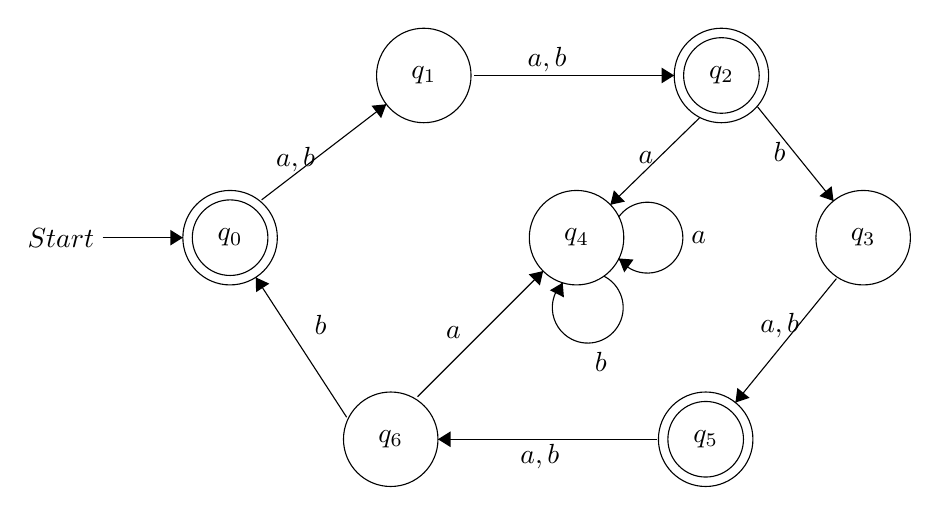
\begin{tikzpicture}[scale=0.2]
\tikzstyle{every node}+=[inner sep=0pt]
\draw [black] (13.6,-25.6) circle (3);
\draw (13.6,-25.6) node {$q_0$};
\draw [black] (13.6,-25.6) circle (2.4);
\draw [black] (25.9,-15.3) circle (3);
\draw (25.9,-15.3) node {$q_1$};
\draw [black] (44.8,-15.3) circle (3);
\draw (44.8,-15.3) node {$q_2$};
\draw [black] (44.8,-15.3) circle (2.4);
\draw [black] (35.6,-25.6) circle (3);
\draw (35.6,-25.6) node {$q_4$};
\draw [black] (53.8,-25.6) circle (3);
\draw (53.8,-25.6) node {$q_3$};
\draw [black] (43.8,-38.4) circle (3);
\draw (43.8,-38.4) node {$q_5$};
\draw [black] (43.8,-38.4) circle (2.4);
\draw [black] (23.8,-38.4) circle (3);
\draw (23.8,-38.4) node {$q_6$};
\draw [black] (5.5,-25.6) -- (10.6,-25.6);
\draw (5,-25.6) node [left] {$Start$};
\fill [black] (10.6,-25.6) -- (9.8,-25.1) -- (9.8,-26.1);
\draw [black] (15.6,-23.2) -- (23.52,-17.13);
\draw (19.03,-20.61) node [left] {$a,b$};
\fill [black] (23.52,-17.13) -- (22.58,-17.22) -- (23.19,-18.01);
\draw [black] (29.1,-15.3) -- (41.8,-15.3);
\draw (35,-14.3) node [left] {$a,b$};
\fill [black] (41.8,-15.3) -- (41,-14.8) -- (41,-15.8);
\draw [black] (47.1,-17.3) -- (51.92,-23.27);
\draw (48.5,-20.81) node [above] {$b$};
\fill [black] (51.92,-23.27) -- (51.8,-22.33) -- (51.02,-22.96);
\draw [black] (52.1,-28.2) -- (45.69,-36.07);
\draw (48.5,-32) node [above] {$a,b$};
\fill [black] (45.69,-36.07) -- (46.59,-35.77) -- (45.81,-35.14);
\draw [black] (40.7,-38.4) -- (26.8,-38.4);
\draw (32,-39.5) node [right] {$a,b$};
\fill [black] (26.8,-38.4) -- (27.6,-38.9) -- (27.6,-37.9);
\draw [black] (21,-37) -- (15.23,-28.12);
\draw (19.35,-30.5) node [below] {$b$};
\fill [black] (15.23,-28.12) -- (15.25,-29.06) -- (16.09,-28.52);
\draw [black] (25.5,-35.7) -- (33.48,-27.72);
\draw (27.78,-31.18) node [below] {$a$};
\fill [black] (33.48,-27.72) -- (32.56,-27.93) -- (33.27,-28.64);
\draw [black] (43.4,-18) -- (37.75,-23.51);
\draw (39.5,-20.53) node [right] {$a$};
\fill [black] (37.75,-23.51) -- (38.67,-23.31) -- (37.97,-22.59);
\draw [black] (38.28,-24.277) arc (144:-144:2.25);
\draw (42.85,-25.6) node [right] {$a$};
\fill [black] (38.28,-26.92) -- (38.63,-27.8) -- (39.22,-26.99);
\draw [black] (37.329,-28.037) arc (63.09028:-224.90972:2.25);
\draw (37.14,-32.87) node [below] {$b$};
\fill [black] (34.72,-28.46) -- (33.91,-28.94) -- (34.8,-29.39);
\end{tikzpicture}
\end{center}

\subsection*{c.}

\begin{center}
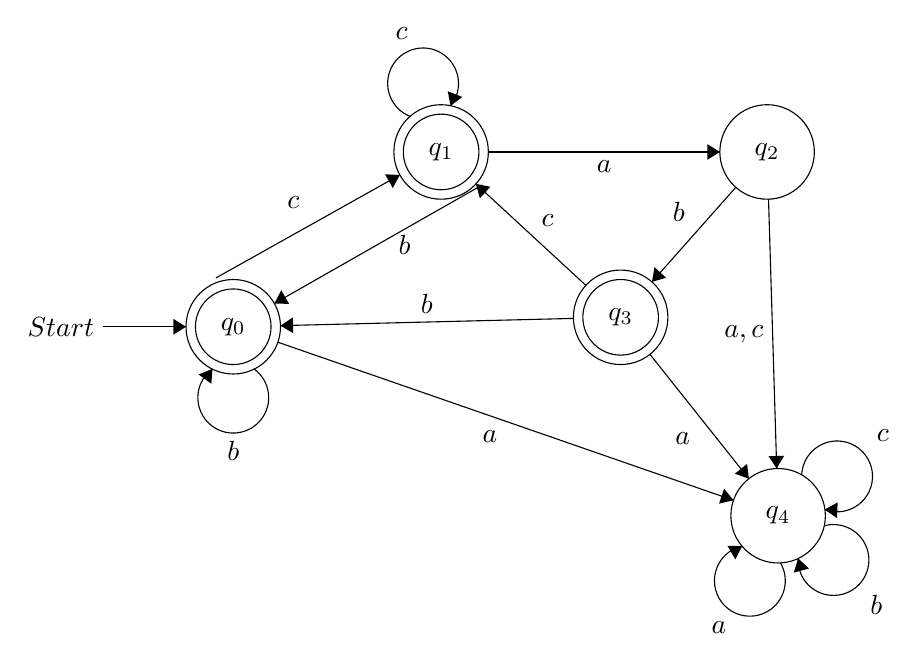
\begin{tikzpicture}[scale=0.2]
\tikzstyle{every node}+=[inner sep=0pt]
\draw [black] (15.9,-24.7) circle (3);
\draw (15.9,-24.7) node {$q_0$};
\draw [black] (15.9,-24.7) circle (2.4);
\draw [black] (29.1,-13.6) circle (3);
\draw (29.1,-13.6) node {$q_1$};
\draw [black] (29.1,-13.6) circle (2.4);
\draw [black] (49.8,-13.6) circle (3);
\draw (49.8,-13.6) node {$q_2$};
\draw [black] (40.5,-24.1) circle (3);
\draw (40.5,-24.1) node {$q_3$};
\draw [black] (40.5,-24.1) circle (2.4);
\draw [black] (50.5,-36.7) circle (3);
\draw (50.5,-36.7) node {$q_4$};
\draw [black] (7.6,-24.7) -- (12.9,-24.7);
\draw (7.1,-24.7) node [left] {$Start$};
\fill [black] (12.9,-24.7) -- (12.1,-24.2) -- (12.1,-25.2);
\draw [black] (17.223,-27.38) arc (54:-234:2.25);
\draw (15.9,-31.95) node [below] {$b$};
\fill [black] (14.58,-27.38) -- (13.7,-27.73) -- (14.51,-28.32);
\draw [black] (14.8,-21.6) -- (26.48,-15.06);
\draw (20.14,-16.81) node [left] {$c$};
\fill [black] (26.48,-15.06) -- (25.54,-15.02) -- (26.03,-15.89);
\draw [black] (31.7,-15.7) -- (18.51,-23.22);
\draw (26.36,-19.48) node [right] {$b$};
\fill [black] (18.51,-23.22) -- (19.45,-23.25) -- (18.95,-22.38);
\draw [black] (27.139,-11.345) arc (248.74356:-39.25644:2.25);
\draw (26.59,-6.5) node [above] {$c$};
\fill [black] (29.7,-10.67) -- (30.45,-10.11) -- (29.52,-9.75);
\draw [black] (32.1,-13.6) -- (46.8,-13.6);
\fill [black] (46.8,-13.6) -- (46,-13.1) -- (46,-14.1);
\draw (39.45,-14.1) node [below] {$a$};
\draw [black] (47.81,-15.85) -- (42.49,-21.85);
\fill [black] (42.49,-21.85) -- (43.39,-21.59) -- (42.65,-20.92);
\draw (44.61,-17.4) node [left] {$b$};
\draw [black] (49.89,-16.6) -- (50.41,-33.7);
\fill [black] (50.41,-33.7) -- (50.88,-32.89) -- (49.89,-32.92);
\draw (49.6,-25.16) node [left] {$a,c$};
\draw [black] (42.36,-26.45) -- (48.64,-34.35);
\fill [black] (48.64,-34.35) -- (48.53,-33.41) -- (47.75,-34.03);
\draw (44.94,-31.82) node [left] {$a$};
\draw [black] (18.73,-25.68) -- (47.67,-35.72);
\fill [black] (47.67,-35.72) -- (47.07,-34.98) -- (46.75,-35.93);
\draw (32.2,-31.24) node [below] {$a$};
\draw [black] (50.644,-39.685) arc (30.50143:-257.49857:2.25);
\draw (46.74,-43.4) node [below] {$a$};
\fill [black] (48.22,-38.63) -- (47.28,-38.61) -- (47.78,-39.47);
\draw [black] (51.996,-34.113) arc (177.69007:-110.30993:2.25);
\draw (56.73,-31.62) node [right] {$c$};
\fill [black] (53.46,-36.31) -- (54.24,-36.85) -- (54.28,-35.85);
\draw [black] (53.419,-37.341) arc (105.34019:-182.65981:2.25);
\draw (56.33,-42.34) node [right] {$b$};
\fill [black] (51.77,-39.41) -- (51.5,-40.31) -- (52.46,-40.05);
\draw [black] (38.29,-22.07) -- (31.31,-15.63);
\fill [black] (31.31,-15.63) -- (31.56,-16.54) -- (32.23,-15.81);
\draw (35.87,-18.36) node [above] {$c$};
\draw [black] (37.5,-24.17) -- (18.9,-24.63);
\fill [black] (18.9,-24.63) -- (19.71,-25.11) -- (19.69,-24.11);
\draw (28.19,-23.87) node [above] {$b$};
\end{tikzpicture}
\end{center}

\section*{Answer 3}

This is the NFA N described in question 3.
\begin{center}
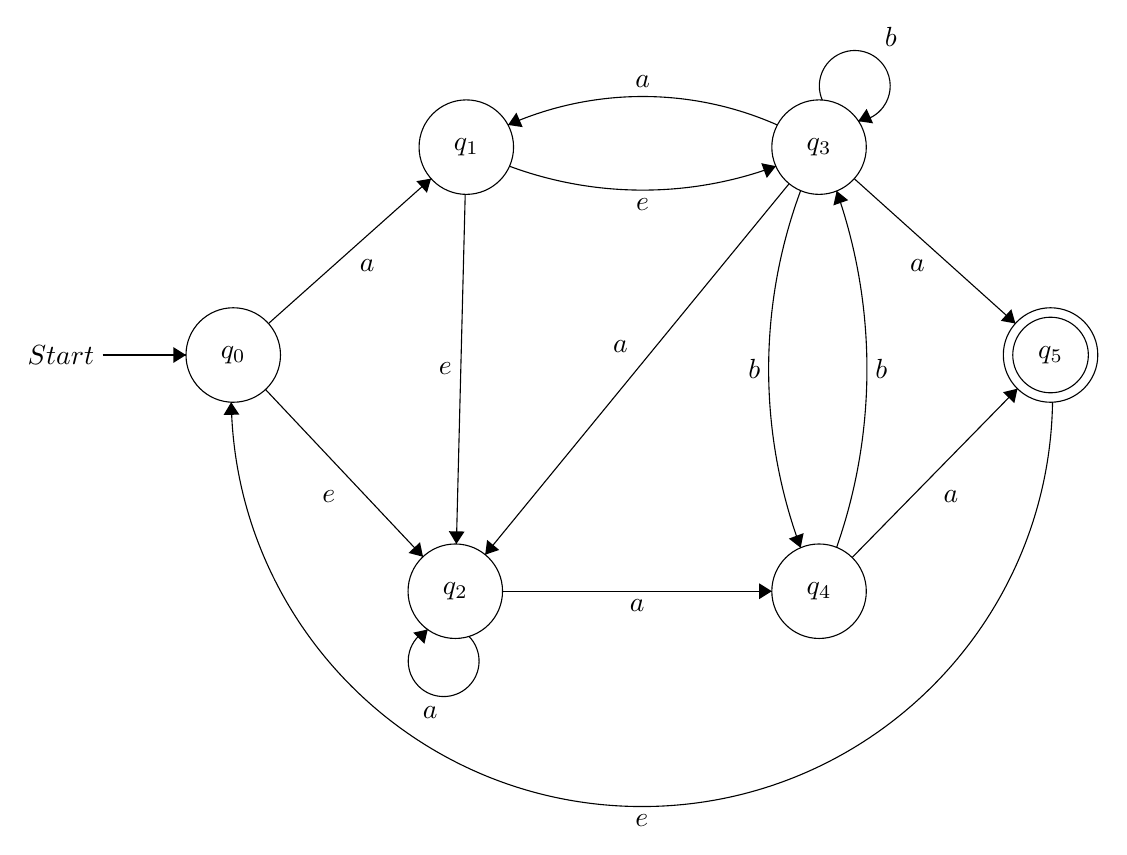
\begin{tikzpicture}[scale=0.2]
\tikzstyle{every node}+=[inner sep=0pt]
\draw [black] (14.3,-27.2) circle (3);
\draw (14.3,-27.2) node {$q_0$};
\draw [black] (29.1,-14) circle (3);
\draw (29.1,-14) node {$q_1$};
\draw [black] (28.4,-42.2) circle (3);
\draw (28.4,-42.2) node {$q_2$};
\draw [black] (51.5,-14) circle (3);
\draw (51.5,-14) node {$q_3$};
\draw [black] (51.5,-42.2) circle (3);
\draw (51.5,-42.2) node {$q_4$};
\draw [black] (66.2,-27.2) circle (3);
\draw (66.2,-27.2) node {$q_5$};
\draw [black] (66.2,-27.2) circle (2.4);
\draw [black] (6,-27.2) -- (11.3,-27.2);
\draw (5.5,-27.2) node [left] {$Start$};
\fill [black] (11.3,-27.2) -- (10.5,-26.7) -- (10.5,-27.7);
\draw [black] (16.54,-25.2) -- (26.86,-16);
\fill [black] (26.86,-16) -- (25.93,-16.16) -- (26.6,-16.9);
\draw (22.81,-21.09) node [below] {$a$};
\draw [black] (16.35,-29.39) -- (26.35,-40.01);
\fill [black] (26.35,-40.01) -- (26.16,-39.09) -- (25.43,-39.77);
\draw (20.82,-36.17) node [left] {$e$};
\draw [black] (29.03,-17) -- (28.47,-39.2);
\fill [black] (28.47,-39.2) -- (28.99,-38.41) -- (27.99,-38.39);
\draw (28.21,-28.09) node [left] {$e$};
\draw [black] (48.758,-15.213) arc (-69.66766:-110.33234:24.343);
\fill [black] (48.76,-15.21) -- (47.83,-15.02) -- (48.18,-15.96);
\draw (40.3,-17.23) node [below] {$e$};
\draw [black] (29.264,-45.061) arc (44.53768:-243.46232:2.25);
\draw (26.81,-49.46) node [below] {$a$};
\fill [black] (26.65,-44.63) -- (25.73,-44.83) -- (26.44,-45.54);
\draw [black] (31.4,-42.2) -- (48.5,-42.2);
\fill [black] (48.5,-42.2) -- (47.7,-41.7) -- (47.7,-42.7);
\draw (39.95,-42.7) node [below] {$a$};
\draw [black] (31.748,-12.594) arc (113.89368:66.10632:21.115);
\fill [black] (31.75,-12.59) -- (32.68,-12.73) -- (32.28,-11.81);
\draw (40.3,-10.28) node [above] {$a$};
\draw [black] (49.6,-16.32) -- (30.3,-39.88);
\fill [black] (30.3,-39.88) -- (31.19,-39.58) -- (30.42,-38.94);
\draw (39.39,-26.67) node [left] {$a$};
\draw [black] (53.73,-16) -- (63.97,-25.2);
\fill [black] (63.97,-25.2) -- (63.71,-24.29) -- (63.04,-25.03);
\draw (57.74,-21.09) node [below] {$a$};
\draw [black] (51.708,-11.019) arc (203.74356:-84.25644:2.25);
\draw (56.05,-7.67) node [above] {$b$};
\fill [black] (53.99,-12.35) -- (54.93,-12.49) -- (54.52,-11.57);
\draw [black] (50.33,-39.439) arc (-159.66495:-200.33505:32.629);
\fill [black] (50.33,-39.44) -- (50.52,-38.51) -- (49.58,-38.86);
\draw (47.8,-28.1) node [left] {$b$};
\draw [black] (53.6,-40.06) -- (64.1,-29.34);
\fill [black] (64.1,-29.34) -- (63.18,-29.56) -- (63.9,-30.26);
\draw (59.38,-36.17) node [right] {$a$};
\draw [black] (52.615,-16.784) arc (19.31526:-19.31526:34.211);
\fill [black] (52.62,-16.78) -- (52.41,-17.7) -- (53.35,-17.37);
\draw (55.04,-28.1) node [right] {$b$};
\draw [black] (66.326,-30.196) arc (-0.88233:-179.11767:26.079);
\fill [black] (14.17,-30.2) -- (13.69,-31) -- (14.69,-30.99);
\draw (40.25,-56.37) node [below] {$e$};
\end{tikzpicture}
\end{center}


\subsection*{a.}
"w1 = abbb"

\begin{center}
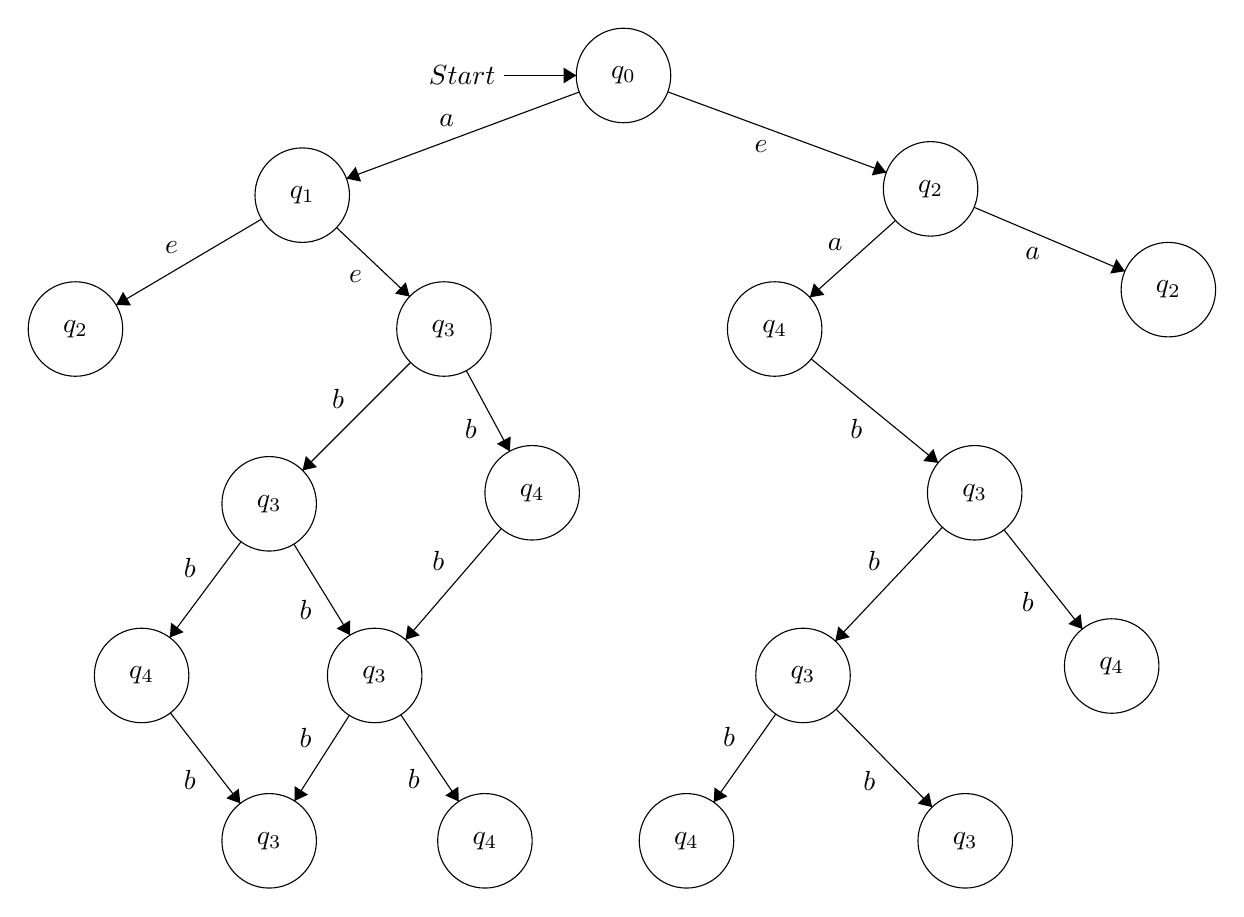
\begin{tikzpicture}[scale=0.2]
\tikzstyle{every node}+=[inner sep=0pt]
\draw [black] (40.6,-3.2) circle (3);
\draw (40.6,-3.2) node {$q_0$};
\draw [black] (20.2,-10.8) circle (3);
\draw (20.2,-10.8) node {$q_1$};
\draw [black] (5.8,-19.3) circle (3);
\draw (5.8,-19.3) node {$q_2$};
\draw [black] (29.2,-19.3) circle (3);
\draw (29.2,-19.3) node {$q_3$};
\draw [black] (18.1,-30.4) circle (3);
\draw (18.1,-30.4) node {$q_3$};
\draw [black] (34.8,-29.7) circle (3);
\draw (34.8,-29.7) node {$q_4$};
\draw [black] (24.8,-41.3) circle (3);
\draw (24.8,-41.3) node {$q_3$};
\draw [black] (10,-41.3) circle (3);
\draw (10,-41.3) node {$q_4$};
\draw [black] (18.1,-51.8) circle (3);
\draw (18.1,-51.8) node {$q_3$};
\draw [black] (31.8,-51.8) circle (3);
\draw (31.8,-51.8) node {$q_4$};
\draw [black] (60.1,-10.4) circle (3);
\draw (60.1,-10.4) node {$q_2$};
\draw [black] (75.2,-16.8) circle (3);
\draw (75.2,-16.8) node {$q_2$};
\draw [black] (50.2,-19.3) circle (3);
\draw (50.2,-19.3) node {$q_4$};
\draw [black] (62.9,-29.7) circle (3);
\draw (62.9,-29.7) node {$q_3$};
\draw [black] (52,-41.3) circle (3);
\draw (52,-41.3) node {$q_3$};
\draw [black] (71.6,-40.7) circle (3);
\draw (71.6,-40.7) node {$q_4$};
\draw [black] (62.3,-51.8) circle (3);
\draw (62.3,-51.8) node {$q_3$};
\draw [black] (44.6,-51.8) circle (3);
\draw (44.6,-51.8) node {$q_4$};
\draw [black] (33,-3.2) -- (37.6,-3.2);
\draw (32.5,-3.2) node [left] {$Start$};
\fill [black] (37.6,-3.2) -- (36.8,-2.7) -- (36.8,-3.7);
\draw [black] (37.79,-4.25) -- (23.01,-9.75);
\fill [black] (23.01,-9.75) -- (23.94,-9.94) -- (23.59,-9);
\draw (29.37,-6.47) node [above] {$a$};
\draw [black] (17.62,-12.32) -- (8.38,-17.78);
\fill [black] (8.38,-17.78) -- (9.33,-17.8) -- (8.82,-16.94);
\draw (11.9,-14.55) node [above] {$e$};
\draw [black] (22.38,-12.86) -- (27.02,-17.24);
\fill [black] (27.02,-17.24) -- (26.78,-16.33) -- (26.09,-17.05);
\draw (23.58,-15.53) node [below] {$e$};
\draw [black] (27.08,-21.42) -- (20.22,-28.28);
\fill [black] (20.22,-28.28) -- (21.14,-28.07) -- (20.43,-27.36);
\draw (22.48,-24.37) node [above] {$b$};
\draw [black] (30.62,-21.94) -- (33.38,-27.06);
\fill [black] (33.38,-27.06) -- (33.44,-26.12) -- (32.56,-26.59);
\draw (31.32,-25.67) node [left] {$b$};
\draw [black] (16.31,-32.81) -- (11.79,-38.89);
\fill [black] (11.79,-38.89) -- (12.67,-38.55) -- (11.87,-37.95);
\draw (13.47,-34.46) node [left] {$b$};
\draw [black] (19.67,-32.96) -- (23.23,-38.74);
\fill [black] (23.23,-38.74) -- (23.24,-37.8) -- (22.38,-38.32);
\draw (20.82,-37.13) node [left] {$b$};
\draw [black] (32.84,-31.97) -- (26.76,-39.03);
\fill [black] (26.76,-39.03) -- (27.66,-38.75) -- (26.9,-38.1);
\draw (29.25,-34.05) node [left] {$b$};
\draw [black] (23.19,-43.83) -- (19.71,-49.27);
\fill [black] (19.71,-49.27) -- (20.57,-48.87) -- (19.72,-48.33);
\draw (20.83,-45.24) node [left] {$b$};
\draw [black] (26.46,-43.8) -- (30.14,-49.3);
\fill [black] (30.14,-49.3) -- (30.11,-48.36) -- (29.28,-48.92);
\draw (27.69,-47.88) node [left] {$b$};
\draw [black] (11.83,-43.68) -- (16.27,-49.42);
\fill [black] (16.27,-49.42) -- (16.17,-48.49) -- (15.38,-49.1);
\draw (13.48,-47.96) node [left] {$b$};
\draw [black] (43.41,-4.24) -- (57.29,-9.36);
\fill [black] (57.29,-9.36) -- (56.71,-8.61) -- (56.36,-9.55);
\draw (49.33,-7.33) node [below] {$e$};
\draw [black] (62.86,-11.57) -- (72.44,-15.63);
\fill [black] (72.44,-15.63) -- (71.9,-14.86) -- (71.51,-15.78);
\draw (66.58,-14.11) node [below] {$a$};
\draw [black] (57.87,-12.41) -- (52.43,-17.29);
\fill [black] (52.43,-17.29) -- (53.36,-17.13) -- (52.69,-16.39);
\draw (54.04,-14.36) node [above] {$a$};
\draw [black] (52.52,-21.2) -- (60.58,-27.8);
\fill [black] (60.58,-27.8) -- (60.28,-26.91) -- (59.64,-27.68);
\draw (55.39,-24.99) node [below] {$b$};
\draw [black] (60.85,-31.89) -- (54.05,-39.11);
\fill [black] (54.05,-39.11) -- (54.97,-38.87) -- (54.24,-38.19);
\draw (56.92,-34.03) node [left] {$b$};
\draw [black] (64.76,-32.05) -- (69.74,-38.35);
\fill [black] (69.74,-38.35) -- (69.63,-37.41) -- (68.85,-38.03);
\draw (66.69,-36.62) node [left] {$b$};
\draw [black] (50.27,-43.75) -- (46.33,-49.35);
\fill [black] (46.33,-49.35) -- (47.2,-48.98) -- (46.38,-48.41);
\draw (47.71,-45.18) node [left] {$b$};
\draw [black] (54.1,-43.44) -- (60.2,-49.66);
\fill [black] (60.2,-49.66) -- (60,-48.74) -- (59.28,-49.44);
\draw (56.62,-48.02) node [left] {$b$};
\end{tikzpicture}
\end{center}

If the string "abbb" is read by this NFA N,as it can be seen in the above diagram which shows all the possibilities,none of the roads lead to accepting final state namely $q_5$.\\

Thus, string "w1=abbb" is not contained by $L(N)$.\\

\subsection*{b.}

"w2 = ababa"

\begin{center}
\begin{tikzpicture}[scale=0.2]
\tikzstyle{every node}+=[inner sep=0pt]
\draw [black] (15.2,-10.5) circle (3);
\draw (15.2,-10.5) node {$q_0$};
\draw [black] (33.9,-10.5) circle (3);
\draw (33.9,-10.5) node {$q_2$};
\draw [black] (56.4,-10.5) circle (3);
\draw (56.4,-10.5) node {$q_4$};
\draw [black] (56.4,-26.4) circle (3);
\draw (56.4,-26.4) node {$q_3$};
\draw [black] (33.9,-26.4) circle (3);
\draw (33.9,-26.4) node {$q_1$};
\draw [black] (15.2,-26.4) circle (3);
\draw (15.2,-26.4) node {$q_3$};
\draw [black] (15.2,-43.8) circle (3);
\draw (15.2,-43.8) node {$q_4$};
\draw [black] (34.9,-43.8) circle (3);
\draw (34.9,-43.8) node {$q_5$};
\draw [black] (34.9,-43.8) circle (2.4);
\draw [black] (6.8,-10.5) -- (12.2,-10.5);
\draw (6.3,-10.5) node [left] {$Start$};
\fill [black] (12.2,-10.5) -- (11.4,-10) -- (11.4,-11);
\draw [black] (18.2,-10.5) -- (30.9,-10.5);
\fill [black] (30.9,-10.5) -- (30.1,-10) -- (30.1,-11);
\draw (24.55,-11) node [below] {$e$};
\draw [black] (36.9,-10.5) -- (53.4,-10.5);
\fill [black] (53.4,-10.5) -- (52.6,-10) -- (52.6,-11);
\draw (45.15,-11) node [below] {$a$};
\draw [black] (56.4,-13.5) -- (56.4,-23.4);
\fill [black] (56.4,-23.4) -- (56.9,-22.6) -- (55.9,-22.6);
\draw (55.9,-18.45) node [left] {$b$};
\draw [black] (53.4,-26.4) -- (36.9,-26.4);
\fill [black] (36.9,-26.4) -- (37.7,-26.9) -- (37.7,-25.9);
\draw (45.15,-25.9) node [above] {$a$};
\draw [black] (30.9,-26.4) -- (18.2,-26.4);
\fill [black] (18.2,-26.4) -- (19,-26.9) -- (19,-25.9);
\draw (24.55,-25.9) node [above] {$e$};
\draw [black] (15.2,-29.4) -- (15.2,-40.8);
\fill [black] (15.2,-40.8) -- (15.7,-40) -- (14.7,-40);
\draw (14.7,-35.1) node [left] {$b$};
\draw [black] (18.2,-43.8) -- (31.9,-43.8);
\fill [black] (31.9,-43.8) -- (31.1,-43.3) -- (31.1,-44.3);
\draw (25.05,-44.3) node [below] {$a$};
\end{tikzpicture}
\end{center}

As can be seen in the above diagram,there exist a path in the NFA N which lead to $q_5$ which is final state by reading the string "w2=ababa".\\

Thus,the string "w2=ababa" is in $L(N)$.\\

\section*{Answer 4}

This is the NFA N described in question 4.

\begin{center}
\begin{tikzpicture}[scale=0.2]
\tikzstyle{every node}+=[inner sep=0pt]
\draw [black] (16.8,-22.7) circle (3);
\draw (16.8,-22.7) node {$q_0$};
\draw [black] (34.9,-38) circle (3);
\draw (34.9,-38) node {$q_2$};
\draw [black] (34.9,-38) circle (2.4);
\draw [black] (34.9,-8.7) circle (3);
\draw (34.9,-8.7) node {$q_1$};
\draw [black] (56.1,-22.7) circle (3);
\draw (56.1,-22.7) node {$q_3$};
\draw [black] (56.1,-22.7) circle (2.4);
\draw [black] (8.4,-22.7) -- (13.8,-22.7);
\draw (7.9,-22.7) node [left] {$Start$};
\fill [black] (13.8,-22.7) -- (13,-22.2) -- (13,-23.2);
\draw [black] (19.17,-20.86) -- (32.53,-10.54);
\fill [black] (32.53,-10.54) -- (31.59,-10.63) -- (32.2,-11.42);
\draw (27.01,-16.2) node [below] {$b$};
\draw [black] (33.595,-35.3) arc (-157.01566:-202.98434:30.603);
\fill [black] (33.6,-35.3) -- (33.74,-34.37) -- (32.82,-34.76);
\draw (30.67,-23.35) node [left] {$a$};
\draw [black] (37.4,-10.35) -- (53.6,-21.05);
\fill [black] (53.6,-21.05) -- (53.2,-20.19) -- (52.65,-21.02);
\draw (44.4,-16.2) node [below] {$e$};
\draw [black] (32.61,-36.06) -- (19.09,-24.64);
\fill [black] (19.09,-24.64) -- (19.38,-25.53) -- (20.02,-24.77);
\draw (26.96,-29.86) node [above] {$a$};
\draw [black] (36.263,-11.371) arc (24.10505:-24.10505:29.331);
\fill [black] (36.26,-11.37) -- (36.13,-12.31) -- (37.05,-11.9);
\draw (39.32,-23.35) node [right] {$b$};
\draw [black] (36.223,-40.68) arc (54:-234:2.25);
\draw (34.9,-45.25) node [below] {$b$};
\fill [black] (33.58,-40.68) -- (32.7,-41.03) -- (33.51,-41.62);
\draw [black] (54.196,-25.018) arc (-41.28893:-67.07524:45.587);
\fill [black] (54.2,-25.02) -- (53.29,-25.29) -- (54.04,-25.95);
\draw (47.77,-32.4) node [below] {$b$};
\draw [black] (37.794,-7.926) arc (99.50508:13.61518:15.726);
\fill [black] (37.79,-7.93) -- (38.67,-8.29) -- (38.5,-7.3);
\draw (50.21,-9.81) node [above] {$b$};
\draw [black] (59.04,-22.165) arc (128.0546:-159.9454:2.25);
\draw (63.36,-25.12) node [right] {$a$};
\fill [black] (58.31,-24.71) -- (58.41,-25.65) -- (59.2,-25.03);
\end{tikzpicture}
\end{center}

\subsection*{a.}

In the GFA,there should exist only 1 start state and 1 accept state.For start state,there is no arrow coming to it and for accepting state,there is no arrow outgoing.So, q4 should be added as starting state and q5 as final state. \\
 
This is the GFA for NFA N:
\begin{center}
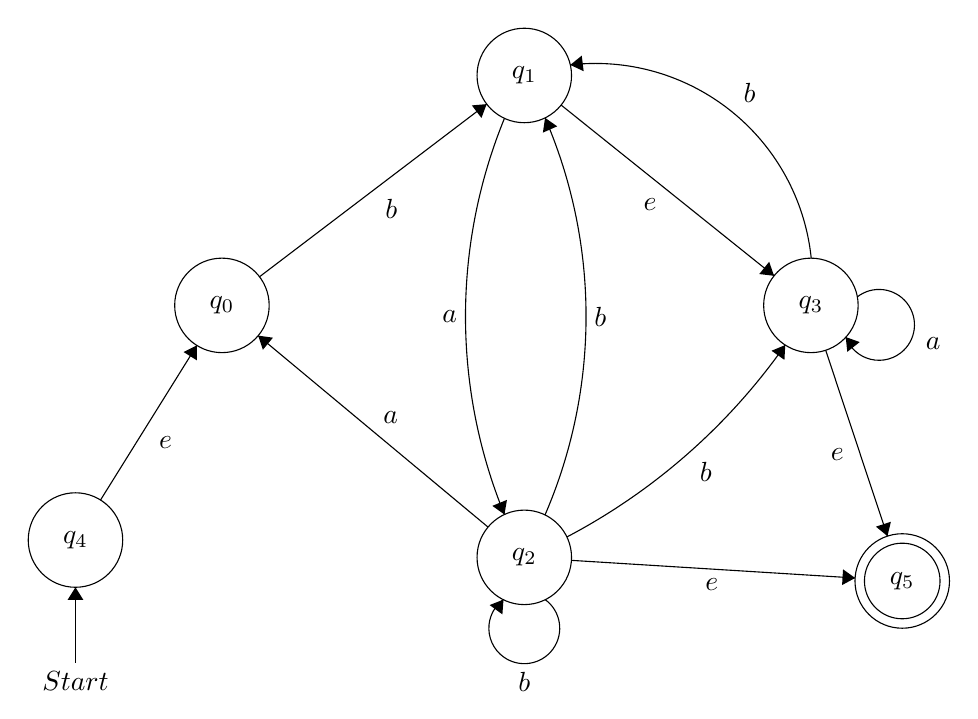
\begin{tikzpicture}[scale=0.2]
\tikzstyle{every node}+=[inner sep=0pt]
\draw [black] (19.4,-22) circle (3);
\draw (19.4,-22) node {$q_0$};
\draw [black] (38.6,-38) circle (3);
\draw (38.6,-38) node {$q_2$};
\draw [black] (38.6,-7.4) circle (3);
\draw (38.6,-7.4) node {$q_1$};
\draw [black] (56.8,-22) circle (3);
\draw (56.8,-22) node {$q_3$};
\draw [black] (10.1,-36.9) circle (3);
\draw (10.1,-36.9) node {$q_4$};
\draw [black] (62.6,-39.5) circle (3);
\draw (62.6,-39.5) node {$q_5$};
\draw [black] (62.6,-39.5) circle (2.4);
\draw [black] (21.79,-20.18) -- (36.21,-9.22);
\fill [black] (36.21,-9.22) -- (35.27,-9.3) -- (35.88,-10.1);
\draw (30.15,-15.2) node [below] {$b$};
\draw [black] (37.34,-35.279) arc (-157.74203:-202.25797:33.208);
\fill [black] (37.34,-35.28) -- (37.5,-34.35) -- (36.57,-34.73);
\draw (34.37,-22.7) node [left] {$a$};
\draw [black] (40.94,-9.28) -- (54.46,-20.12);
\fill [black] (54.46,-20.12) -- (54.15,-19.23) -- (53.52,-20.01);
\draw (46.59,-15.19) node [below] {$e$};
\draw [black] (36.3,-36.08) -- (21.7,-23.92);
\fill [black] (21.7,-23.92) -- (22,-24.82) -- (22.64,-24.05);
\draw (30.11,-29.51) node [above] {$a$};
\draw [black] (39.917,-10.094) arc (23.35686:-23.35686:31.797);
\fill [black] (39.92,-10.09) -- (39.78,-11.03) -- (40.69,-10.63);
\draw (43.02,-22.7) node [right] {$b$};
\draw [black] (39.923,-40.68) arc (54:-234:2.25);
\draw (38.6,-45.25) node [below] {$b$};
\fill [black] (37.28,-40.68) -- (36.4,-41.03) -- (37.21,-41.62);
\draw [black] (55.17,-24.518) arc (-35.09789:-62.26336:39.302);
\fill [black] (55.17,-24.52) -- (54.3,-24.88) -- (55.12,-25.46);
\draw (50.13,-31.93) node [below] {$b$};
\draw [black] (41.518,-6.73) arc (96.68679:5.8402:13.771);
\fill [black] (41.52,-6.73) -- (42.37,-7.13) -- (42.25,-6.14);
\draw (52.9,-9.17) node [above] {$b$};
\draw [black] (59.74,-21.465) arc (128.0546:-159.9454:2.25);
\draw (64.06,-24.42) node [right] {$a$};
\fill [black] (59.01,-24.01) -- (59.11,-24.95) -- (59.9,-24.33);
\draw [black] (11.69,-34.36) -- (17.81,-24.54);
\fill [black] (17.81,-24.54) -- (16.96,-24.96) -- (17.81,-25.49);
\draw (15.38,-30.74) node [right] {$e$};
\draw [black] (10.1,-44.7) -- (10.1,-39.9);
\draw (10.1,-45.2) node [below] {$Start$};
\fill [black] (10.1,-39.9) -- (9.6,-40.7) -- (10.6,-40.7);
\draw [black] (41.59,-38.19) -- (59.61,-39.31);
\fill [black] (59.61,-39.31) -- (58.84,-38.76) -- (58.78,-39.76);
\draw (50.51,-39.31) node [below] {$e$};
\draw [black] (57.74,-24.85) -- (61.66,-36.65);
\fill [black] (61.66,-36.65) -- (61.88,-35.74) -- (60.93,-36.05);
\draw (58.93,-31.45) node [left] {$e$};
\end{tikzpicture}
\end{center}

\subsection*{b.}
1- Elimination of $q_0$ is:

\begin{center}
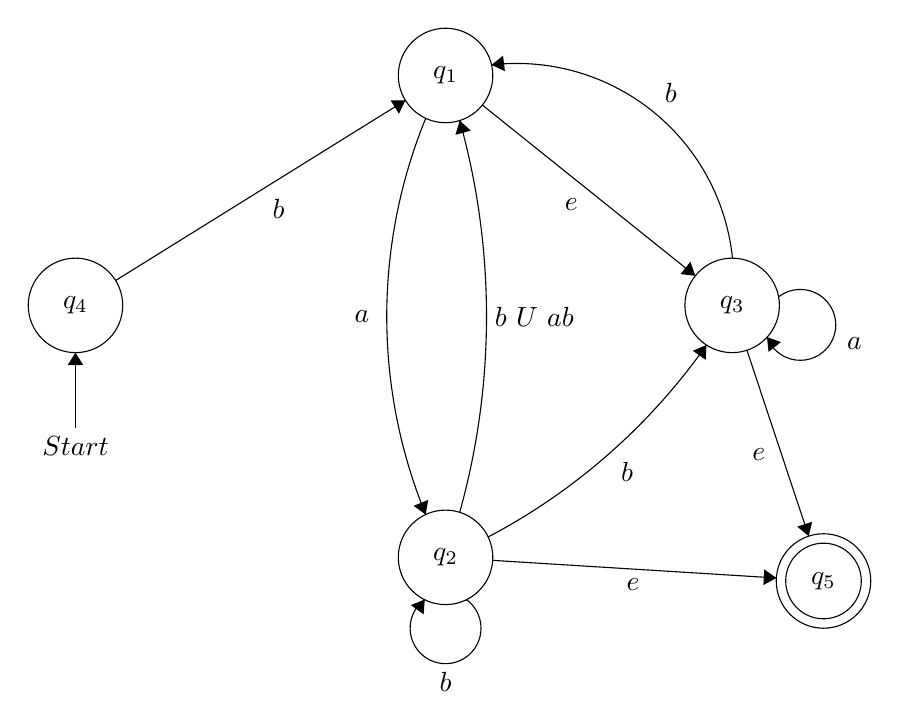
\begin{tikzpicture}[scale=0.2]
\tikzstyle{every node}+=[inner sep=0pt]
\draw [black] (38.6,-38) circle (3);
\draw (38.6,-38) node {$q_2$};
\draw [black] (38.6,-7.4) circle (3);
\draw (38.6,-7.4) node {$q_1$};
\draw [black] (56.8,-22) circle (3);
\draw (56.8,-22) node {$q_3$};
\draw [black] (15.1,-22) circle (3);
\draw (15.1,-22) node {$q_4$};
\draw [black] (62.6,-39.5) circle (3);
\draw (62.6,-39.5) node {$q_5$};
\draw [black] (62.6,-39.5) circle (2.4);
\draw [black] (37.34,-35.279) arc (-157.74203:-202.25797:33.208);
\fill [black] (37.34,-35.28) -- (37.5,-34.35) -- (36.57,-34.73);
\draw (34.37,-22.7) node [left] {$a\mbox{ }$};
\draw [black] (40.94,-9.28) -- (54.46,-20.12);
\fill [black] (54.46,-20.12) -- (54.15,-19.23) -- (53.52,-20.01);
\draw (46.59,-15.19) node [below] {$e$};
\draw [black] (39.499,-10.262) arc (15.58349:-15.58349:46.301);
\fill [black] (39.5,-10.26) -- (39.23,-11.17) -- (40.2,-10.9);
\draw (41.7,-22.7) node [right] {$b\mbox{ }U\mbox{ }ab$};
\draw [black] (39.923,-40.68) arc (54:-234:2.25);
\draw (38.6,-45.25) node [below] {$b$};
\fill [black] (37.28,-40.68) -- (36.4,-41.03) -- (37.21,-41.62);
\draw [black] (55.17,-24.518) arc (-35.09789:-62.26336:39.302);
\fill [black] (55.17,-24.52) -- (54.3,-24.88) -- (55.12,-25.46);
\draw (50.13,-31.93) node [below] {$b$};
\draw [black] (41.518,-6.73) arc (96.68679:5.8402:13.771);
\fill [black] (41.52,-6.73) -- (42.37,-7.13) -- (42.25,-6.14);
\draw (52.9,-9.17) node [above] {$b$};
\draw [black] (59.74,-21.465) arc (128.0546:-159.9454:2.25);
\draw (64.06,-24.42) node [right] {$a$};
\fill [black] (59.01,-24.01) -- (59.11,-24.95) -- (59.9,-24.33);
\draw [black] (15.1,-29.8) -- (15.1,-25);
\draw (15.1,-30.3) node [below] {$Start$};
\fill [black] (15.1,-25) -- (14.6,-25.8) -- (15.6,-25.8);
\draw [black] (41.59,-38.19) -- (59.61,-39.31);
\fill [black] (59.61,-39.31) -- (58.84,-38.76) -- (58.78,-39.76);
\draw (50.51,-39.31) node [below] {$e$};
\draw [black] (57.74,-24.85) -- (61.66,-36.65);
\fill [black] (61.66,-36.65) -- (61.88,-35.74) -- (60.93,-36.05);
\draw (58.93,-31.45) node [left] {$e$};
\draw [black] (17.65,-20.42) -- (36.05,-8.98);
\fill [black] (36.05,-8.98) -- (35.11,-8.98) -- (35.64,-9.83);
\draw (28,-15.2) node [below] {$b$};
\end{tikzpicture}
\end{center}

2- Elimination of $q_1$ is:

\begin{center}
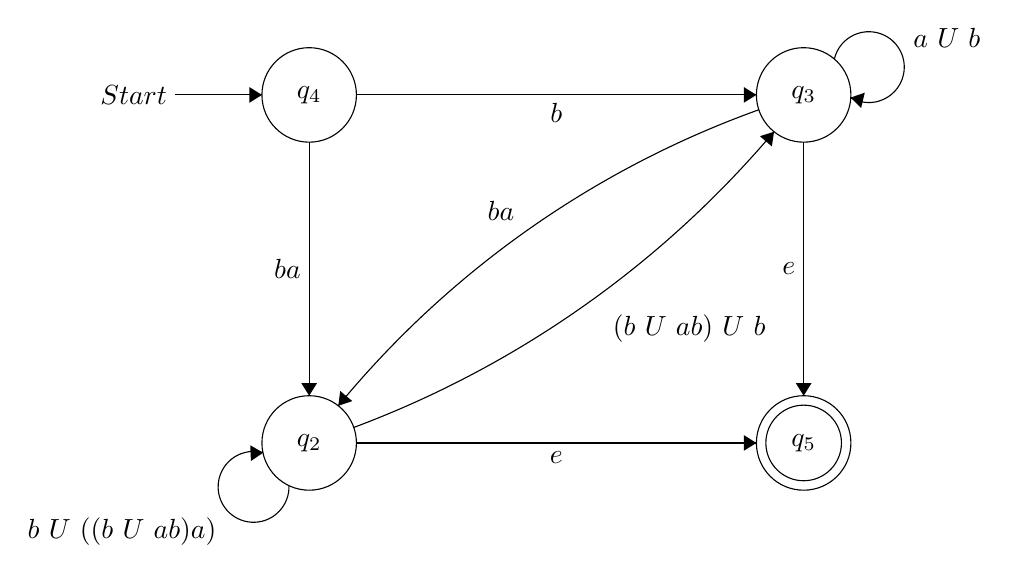
\begin{tikzpicture}[scale=0.2]
\tikzstyle{every node}+=[inner sep=0pt]
\draw [black] (26.4,-40.3) circle (3);
\draw (26.4,-40.3) node {$q_2$};
\draw [black] (57.8,-18.2) circle (3);
\draw (57.8,-18.2) node {$q_3$};
\draw [black] (26.4,-18.2) circle (3);
\draw (26.4,-18.2) node {$q_4$};
\draw [black] (57.8,-40.3) circle (3);
\draw (57.8,-40.3) node {$q_5$};
\draw [black] (57.8,-40.3) circle (2.4);
\draw [black] (25.116,-42.998) arc (2.28024:-285.71976:2.25);
\draw (20.54,-45.9) node [left] {$b\mbox{ }U\mbox{ }((b\mbox{ }U\mbox{ }ab)a)$};
\fill [black] (23.48,-40.92) -- (22.66,-40.45) -- (22.7,-41.45);
\draw [black] (55.917,-20.535) arc (-40.21279:-69.50978:64.514);
\fill [black] (55.92,-20.54) -- (55.02,-20.82) -- (55.78,-21.47);
\draw (50.53,-32.14) node [below] {$(b\mbox{ }U\mbox{ }ab)\mbox{ }U\mbox{ }b$};
\draw [black] (59.746,-15.933) arc (167.0896:-120.9104:2.25);
\draw (64.74,-14.6) node [right] {$a\mbox{ }U\mbox{ }b$};
\fill [black] (60.78,-18.37) -- (61.45,-19.03) -- (61.68,-18.06);
\draw [black] (17.9,-18.2) -- (23.4,-18.2);
\draw (17.4,-18.2) node [left] {$Start$};
\fill [black] (23.4,-18.2) -- (22.6,-17.7) -- (22.6,-18.7);
\draw [black] (29.4,-40.3) -- (54.8,-40.3);
\fill [black] (54.8,-40.3) -- (54,-39.8) -- (54,-40.8);
\draw (42.1,-40.8) node [below] {$e$};
\draw [black] (57.8,-21.2) -- (57.8,-37.3);
\fill [black] (57.8,-37.3) -- (58.3,-36.5) -- (57.3,-36.5);
\draw (57.3,-29.25) node [left] {$e$};
\draw [black] (29.4,-18.2) -- (54.8,-18.2);
\fill [black] (54.8,-18.2) -- (54,-17.7) -- (54,-18.7);
\draw (42.1,-18.7) node [below] {$b$};
\draw [black] (26.4,-21.2) -- (26.4,-37.3);
\fill [black] (26.4,-37.3) -- (26.9,-36.5) -- (25.9,-36.5);
\draw (25.9,-29.25) node [left] {$ba$};
\draw [black] (28.25,-37.938) arc (140.53605:109.74137:61.493);
\fill [black] (28.25,-37.94) -- (29.14,-37.64) -- (28.37,-37);
\draw (38.58,-26.24) node [above] {$ba$};
\end{tikzpicture}
\end{center}

3- Elimination of $q_2$ is:

\begin{center}
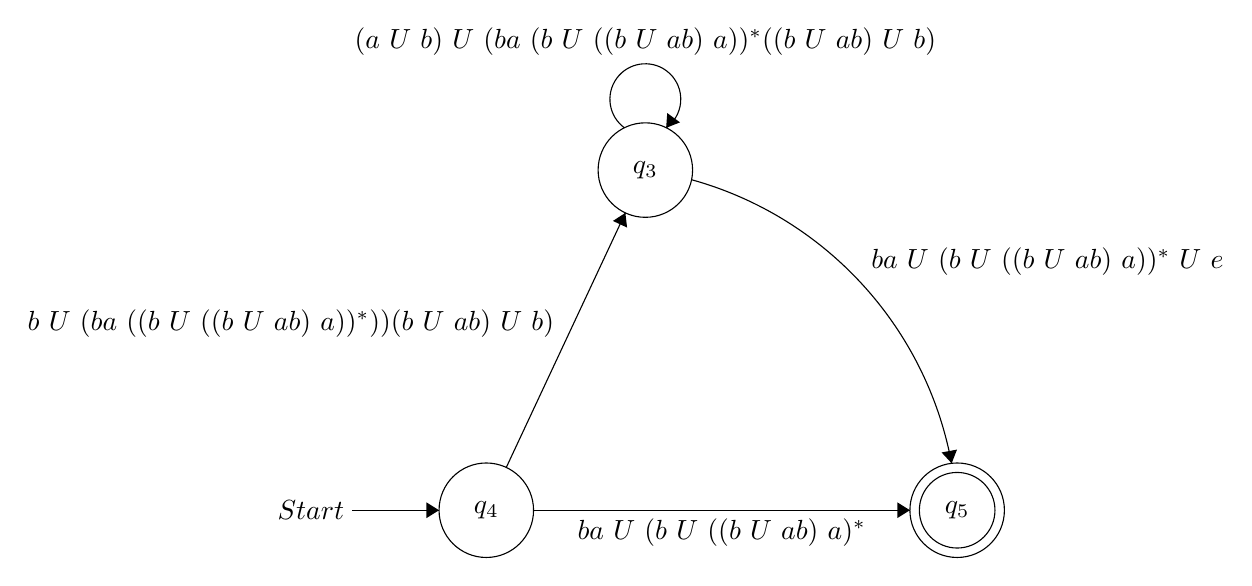
\begin{tikzpicture}[scale=0.2]
\tikzstyle{every node}+=[inner sep=0pt]
\draw [black] (42,-14.8) circle (3);
\draw (42,-14.8) node {$q_3$};
\draw [black] (31.9,-36.4) circle (3);
\draw (31.9,-36.4) node {$q_4$};
\draw [black] (61.8,-36.4) circle (3);
\draw (61.8,-36.4) node {$q_5$};
\draw [black] (61.8,-36.4) circle (2.4);
\draw [black] (40.677,-12.12) arc (234:-54:2.25);
\draw (42,-7.55) node [above] {$(a\mbox{ }U\mbox{ }b)\mbox{ }U\mbox{ }(ba\mbox{ }(b\mbox{ }U\mbox{ }((b\mbox{ }U\mbox{ }ab)\mbox{ }a))^*((b\mbox{ }U\mbox{ }ab)\mbox{ }U\mbox{ }b)$};
\fill [black] (43.32,-12.12) -- (44.2,-11.77) -- (43.39,-11.18);
\draw [black] (23.4,-36.4) -- (28.9,-36.4);
\draw (22.9,-36.4) node [left] {$Start$};
\fill [black] (28.9,-36.4) -- (28.1,-35.9) -- (28.1,-36.9);
\draw [black] (44.935,-15.412) arc (74.49929:10.5216:23.061);
\fill [black] (61.45,-33.42) -- (61.79,-32.55) -- (60.81,-32.73);
\draw (56.31,-20.59) node [right] {$ba\mbox{ }U\mbox{ }(b\mbox{ }U\mbox{ }((b\mbox{ }U\mbox{ }ab)\mbox{ }a))^*\mbox{ }U\mbox{ }e$};
\draw [black] (33.17,-33.68) -- (40.73,-17.52);
\fill [black] (40.73,-17.52) -- (39.94,-18.03) -- (40.84,-18.45);
\draw (36.24,-24.56) node [left] {$b\mbox{ }U\mbox{ }(ba\mbox{ }((b\mbox{ }U\mbox{ }((b\mbox{ }U\mbox{ }ab)\mbox{ }a))^*))(b\mbox{ }U\mbox{ }ab)\mbox{ }U\mbox{ }b)$};
\draw [black] (34.9,-36.4) -- (58.8,-36.4);
\fill [black] (58.8,-36.4) -- (58,-35.9) -- (58,-36.9);
\draw (46.85,-36.9) node [below] {$ba\mbox{ }U\mbox{ }(b\mbox{ }U\mbox{ }((b\mbox{ }U\mbox{ }ab)\mbox{ }a)^*$};
\end{tikzpicture}
\end{center}

4- Elimination of $q_3$ yields to regular expression:

$(ba \cup (b \cup ((b \cup ab)a)^*) \cup (b \cup ( ba(( b \cup (( b \cup ab)a))^*))((b \cup ab) \cup b))((a \cup b) U (ba(b \cup ((b \cup ab)a))^*((b \cup ab) \cup b))^*ba \cup (b \cup ((b \cup ab)a))* \cup e)  $

\section*{Answer 5}

\subsection*{a.}

This is the NFA N :

\begin{center}
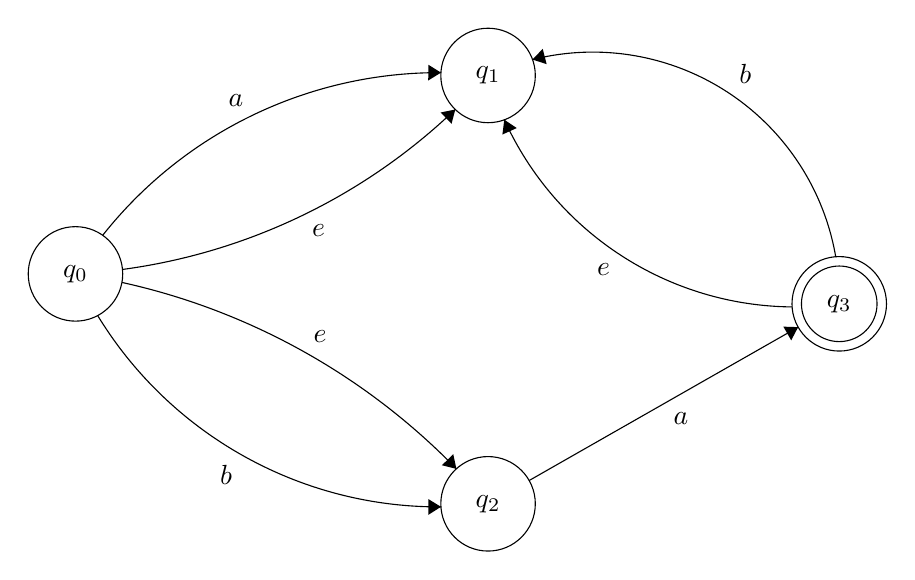
\begin{tikzpicture}[scale=0.2]
\tikzstyle{every node}+=[inner sep=0pt]
\draw [black] (11.1,-25.4) circle (3);
\draw (11.1,-25.4) node {$q_0$};
\draw [black] (37.3,-12.8) circle (3);
\draw (37.3,-12.8) node {$q_1$};
\draw [black] (37.3,-40) circle (3);
\draw (37.3,-40) node {$q_2$};
\draw [black] (59.6,-27.3) circle (3);
\draw (59.6,-27.3) node {$q_3$};
\draw [black] (59.6,-27.3) circle (2.4);
\draw [black] (12.829,-22.95) arc (141.63755:89.72975:27.228);
\fill [black] (34.31,-12.62) -- (33.51,-12.12) -- (33.5,-13.12);
\draw (21.29,-14.8) node [above] {$a$};
\draw [black] (35.216,-14.957) arc (-46.27401:-82.35869:37.852);
\fill [black] (35.22,-14.96) -- (34.29,-15.15) -- (34.98,-15.87);
\draw (26.54,-22.22) node [below] {$e$};
\draw [black] (34.308,-40.194) arc (-89.67597:-148.58167:25.376);
\fill [black] (34.31,-40.19) -- (33.51,-39.7) -- (33.51,-40.7);
\draw (20.67,-37.49) node [below] {$b$};
\draw [black] (14.05,-25.942) arc (77.55826:44.1841:42.334);
\fill [black] (35.29,-37.78) -- (35.09,-36.85) -- (34.37,-37.55);
\draw (26.63,-29.8) node [above] {$e$};
\draw [black] (39.91,-38.52) -- (56.99,-28.78);
\fill [black] (56.99,-28.78) -- (56.05,-28.75) -- (56.55,-29.62);
\draw (49.55,-34.15) node [below] {$a$};
\draw [black] (40.121,-11.792) arc (104.1728:9.76141:15.651);
\fill [black] (40.12,-11.79) -- (41.02,-12.08) -- (40.77,-11.11);
\draw (53.64,-13.35) node [above] {$b$};
\draw [black] (56.609,-27.497) arc (-90.48073:-155.58506:20.257);
\fill [black] (38.33,-15.61) -- (38.21,-16.55) -- (39.12,-16.14);
\draw (44.64,-24.72) node [below] {$e$};
\end{tikzpicture}
\end{center} 
$E(q_0) = \{q_0,q_1,q_2\}$\\
$E(q_1) = \{q_1\}$\\
$E(q_2) = \{q_2\}$\\
$E(q_3) = \{q_1,q_3\}$\\
$ \delta (E(q_0),a) = \delta(\{q_0,q_1,q_2\},a)$ = $\{q_1,q_3\}$\\
$ \delta (E(q_0),b) = \delta(\{q_0,q_1,q_2\},b)$ = $\{q_2\}$\\
$ \delta(\{q_1,q_3\},a)$ = $\{\}$\\
$ \delta(\{q_1,q_3\},b)$ = $\{q_1\}$\\
$ \delta(\{q_2\},a)$ = $\{q_3\}$\\
$ \delta(\{q_2\},b)$ = $\{\}$\\
$ \delta(\{q_1\},a)$ = $\{\}$\\
$ \delta(\{q_1\},b)$ = $\{\}$\\

So,the equal DFA M for the NFA N is:

\begin{center}
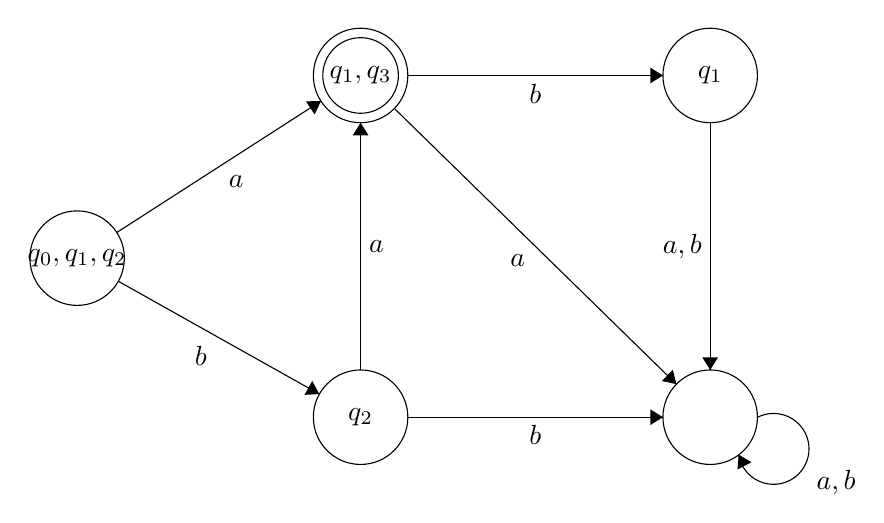
\begin{tikzpicture}[scale=0.2]
\tikzstyle{every node}+=[inner sep=0pt]
\draw [black] (13.5,-25.2) circle (3);
\draw (13.5,-25.2) node {$q_0,q_1,q_2$};
\draw [black] (31.5,-13.6) circle (3);
\draw (31.5,-13.6) node {$q_1,q_3$};
\draw [black] (31.5,-13.6) circle (2.4);
\draw [black] (31.5,-35.3) circle (3);
\draw (31.5,-35.3) node {$q_2$};
\draw [black] (53.7,-13.6) circle (3);
\draw (53.7,-13.6) node {$q_1$};
\draw [black] (53.7,-35.3) circle (3);
\draw (53.7,-35.3) node {${}$};
\draw [black] (16.02,-23.57) -- (28.98,-15.23);
\fill [black] (28.98,-15.23) -- (28.03,-15.24) -- (28.58,-16.08);
\draw (23.6,-19.9) node [below] {$a$};
\draw [black] (16.12,-26.67) -- (28.88,-33.83);
\fill [black] (28.88,-33.83) -- (28.43,-33) -- (27.94,-33.88);
\draw (21.35,-30.75) node [below] {$b$};
\draw [black] (31.5,-32.3) -- (31.5,-16.6);
\fill [black] (31.5,-16.6) -- (31,-17.4) -- (32,-17.4);
\draw (32,-24.45) node [right] {$a$};
\draw [black] (34.5,-13.6) -- (50.7,-13.6);
\fill [black] (50.7,-13.6) -- (49.9,-13.1) -- (49.9,-14.1);
\draw (42.6,-14.1) node [below] {$b$};
\draw [black] (33.65,-15.7) -- (51.55,-33.2);
\fill [black] (51.55,-33.2) -- (51.33,-32.29) -- (50.63,-33);
\draw (41.48,-24.93) node [below] {$a$};
\draw [black] (53.7,-16.6) -- (53.7,-32.3);
\fill [black] (53.7,-32.3) -- (54.2,-31.5) -- (53.2,-31.5);
\draw (53.2,-24.45) node [left] {$a,b$};
\draw [black] (34.5,-35.3) -- (50.7,-35.3);
\fill [black] (50.7,-35.3) -- (49.9,-34.8) -- (49.9,-35.8);
\draw (42.6,-35.8) node [below] {$b$};
\draw [black] (56.688,-35.316) arc (117.43495:-170.56505:2.25);
\draw (60.43,-39.43) node [right] {$a,b$};
\fill [black] (55.51,-37.68) -- (55.43,-38.62) -- (56.32,-38.16);
\end{tikzpicture}
\end{center}

\subsection*{b.}

The compelement of a DFA is obtained by changing the final states by nonfinal states and nonfinal states by final states.

\begin{center}
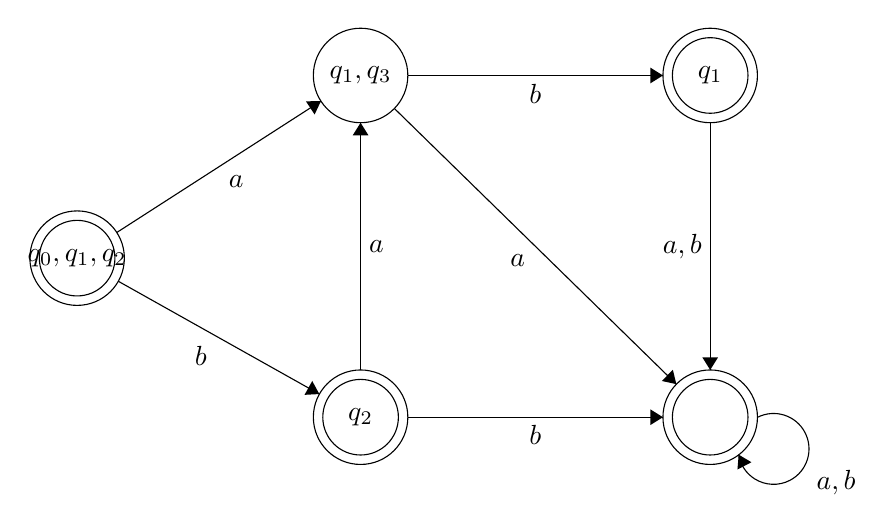
\begin{tikzpicture}[scale=0.2]
\tikzstyle{every node}+=[inner sep=0pt]
\draw [black] (13.5,-25.2) circle (3);
\draw (13.5,-25.2) node {$q_0,q_1,q_2$};
\draw [black] (13.5,-25.2) circle (2.4);
\draw [black] (31.5,-13.6) circle (3);
\draw (31.5,-13.6) node {$q_1,q_3$};
\draw [black] (31.5,-35.3) circle (3);
\draw (31.5,-35.3) node {$q_2$};
\draw [black] (31.5,-35.3) circle (2.4);
\draw [black] (53.7,-13.6) circle (3);
\draw (53.7,-13.6) node {$q_1$};
\draw [black] (53.7,-13.6) circle (2.4);
\draw [black] (53.7,-35.3) circle (3);
\draw (53.7,-35.3) node {${}$};
\draw [black] (53.7,-35.3) circle (2.4);
\draw [black] (16.02,-23.57) -- (28.98,-15.23);
\fill [black] (28.98,-15.23) -- (28.03,-15.24) -- (28.58,-16.08);
\draw (23.6,-19.9) node [below] {$a$};
\draw [black] (16.12,-26.67) -- (28.88,-33.83);
\fill [black] (28.88,-33.83) -- (28.43,-33) -- (27.94,-33.88);
\draw (21.35,-30.75) node [below] {$b$};
\draw [black] (31.5,-32.3) -- (31.5,-16.6);
\fill [black] (31.5,-16.6) -- (31,-17.4) -- (32,-17.4);
\draw (32,-24.45) node [right] {$a$};
\draw [black] (34.5,-13.6) -- (50.7,-13.6);
\fill [black] (50.7,-13.6) -- (49.9,-13.1) -- (49.9,-14.1);
\draw (42.6,-14.1) node [below] {$b$};
\draw [black] (33.65,-15.7) -- (51.55,-33.2);
\fill [black] (51.55,-33.2) -- (51.33,-32.29) -- (50.63,-33);
\draw (41.48,-24.93) node [below] {$a$};
\draw [black] (53.7,-16.6) -- (53.7,-32.3);
\fill [black] (53.7,-32.3) -- (54.2,-31.5) -- (53.2,-31.5);
\draw (53.2,-24.45) node [left] {$a,b$};
\draw [black] (34.5,-35.3) -- (50.7,-35.3);
\fill [black] (50.7,-35.3) -- (49.9,-34.8) -- (49.9,-35.8);
\draw (42.6,-35.8) node [below] {$b$};
\draw [black] (56.688,-35.316) arc (117.43495:-170.56505:2.25);
\draw (60.43,-39.43) node [right] {$a,b$};
\fill [black] (55.51,-37.68) -- (55.43,-38.62) -- (56.32,-38.16);
\end{tikzpicture}
\end{center}

$\bar{L} = \Sigma^* - L$ $\equiv$ $\bar{L}=\{w|w\in \Sigma^* \wedge w\notin L\}$ 

REgular Expression for DFA M : $(aaa^*b^*)^* \cup (aba^*b^*)^* \cup (baaa^*b^*)^* \cup (baba^*b^*)^*$

$\bar{L}$ using Kleene star,union,concatenation and complement set notation.
\section*{Answer 6}
For any two arbitrary regular languages $L_1$ and $L_2$,there exist NFAs.\\
NFA for $L_1$ is $N_1=\{K_1,\Sigma,\Delta_1,s_1,F_1\}$ and \\ NFA for $L_2$ is $N_2=\{K_2,\Sigma,\Delta_2,s_2,F_2\}$.\\
$L_1-L_2$ = $L_1 \cap \bar{L_2}$.Also $(L_1\cap \bar{L_2})'$ = $\bar{L_1} \cup L_2$.(By De Morgan Laws).\\
Now,it is turned out to be union operation.\\
There exist corresponding DFAs for NFA $N_1$ and $N_2$.By subset construction algorithm,it can be found.Why we take corresponding DFAs is to take complement of these DFAs.\\
DFA $M_1=\{K_1',\Sigma,\delta_1,s_1,F_1'\}$ and \\   
DFA $M_2=\{K_2',\Sigma,\delta_2,s_2,F_2'\}$.
The complement of DFA $M_1$ is $\bar{M_1}=\{K_1',\Sigma,\delta_1,s_1,(F_1')'\}$.\\If union operation is applied to $\bar{M_1}$ and $M_2$,the obtained language is still regular since there exist an NFA for it.
NFA M' $=\{K_1' \cup K_2 \cup q_0,\Sigma,\Delta_1 \cup \Delta_2,q_0,F_1'\}$ where $q_0$ is a new starting state and has e transitions to starting state of $\bar{M_1}$ and $M_2$.\\
Now,NFA M' is for $\bar{L_1} \cup L_2$.If we again use subset construction algorithm,we are able to find the equivalent DFA for NFA M';\\
DFA $(M')'= \{K_1' \cup K_2 \cup q_0,\Sigma,\delta_1' \cup \delta_2',q_0,F_1'\}$.\\
By De Morgan Laws,$\bar{L_1} \cup L_2$ = $(L_1\cap \bar{L_2})'$.\\
If we take the complement of this DFA,we obtain a DFA $= \{K_1' \cup K_2 \cup q_0,\Sigma,\delta_1' \cup \delta_2',q_0,(F_1')'\}$.\\ 
Since $L_1-L_2$ = $L_1 \cap \bar{L_2}$, there exist a finite state automaton for language $L_1-L_2$.Thus,the language $L_1-L_2$ is regular under set difference opertaion.

  



\section*{Answer 7}

\subsection*{a.}

Assume language L is regular.Then there exist an integer called pumping length $p \geq 1$ and every string in L of length at least p can be pumped.By pumping lemma,a string w can be split into 3 parts namely x,y,z and these parts should satisfy following conditions:\\
1-$|y|\geq 1$ \\
2-$|xy|\leq p$ and \\
3-$xy^nz \in L$ for all $n \geq 1$. \\  

Back to the question,assume that language L is regular and let word w is "$a^{p^2}b^p$".Since number of a's in w is $p^2$ and p is integer $\geq 1$ ,w is in L.\\

This word can be split as x = "$a^q$",y="$a^r$" and z="$a^s+b^p$" such that q+r+s = $p^2$, q+r$\leq$ p and r$\geq$1.\\
By looking these (x,y,z),this groupping satisfies 1 and 2.(The length of y is r and length of xy is less than p.)\\
However, if n is chosen as 2,then the string becomes $xy^2z$, $x = "a^q",y="a^{2r}"$ and $z="a^s+b^p"$, $a^{q+2r+s}b^p = a^{p^2+r}b^p$.\\

Since r is less than p becasuse $|xy|\leq p$ and $p^2$ is perfect square of  integer p,$p^2+r$ is not a perfect squre of some natural number N(Since$(p+1)^2-p^2 = 2p+1$ and $p^2+r < (p+1)^2$).Thus,in the $a^{p^2+r}b^p$ string,the number of occurrences of a is not a square of some natural number N and this shows that language L is not a regular language.  



\end{document}

​

